\subsection{การเชื่อมต่อหุ่นยนต์ฮิวมานอยด์}
โครงสร้างแพลตฟอร์มหุ่นยนต์อุทัยจะประกอบไปด้วยสองขา เพื่อทำให้เกิดองศาอิสระเป็น 12 องศาอิสระ
(DOFs) ใช้ Dynamixel servos 12 ตัว มอเตอร์ Dynamixel ทั้งหมดเชื่อมต่อกันแบบ daisy chain
ข้างนึงของมอเตอร์ตัวแรกเชื่อมต่อกับแบตเตอร์รี่ 12V และอีกข้างต่อกับ USB2Dynamixel
ทั้งหมดนี้เป็นการเชื่อมต่อ Odroid เข้ากับหุ่นยนต์ ดังรูปที่ \ref{fig:odroid2dynamixel}

\begin{figure}[htbp]
    \centering
    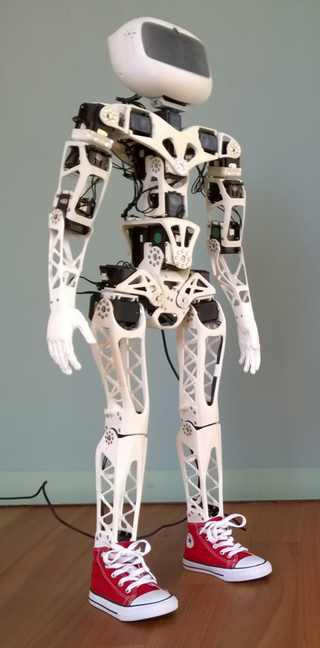
\includegraphics[width=0.3\textwidth]{chapter2/images/PoppyHumanoid1.png}
    \caption{การเชื่อมต่อระหว่าง Odroid กับ Dynamixel servos}
    \label{fig:odroid2dynamixel}
\end{figure}

หุ่นยนต์ฮิวมานอยด์อุทัยใช้เซอร์โวมอเตอร์ 12 ตัว ทำให้เกิดเป็น 12 องศาอิสระ
USB2Dynamixel ใช้เพื่อที่จะสั่งการเซอร์โวมอเตอร์ Dynamixel ผ่าน Odroid
ตำแหน่งของเซอร์โวมอเตอร์ Dynamixel EX-106+ นั้นมาจากเอนโคดเดอร์ที่อยู่ภายใน
เซนเซอร์ Gyro/Accelerometer ติดอยู่กับตัวของหุ่นยนต์ เพื่อช่วยในการทรงตัวของหุ่นยนต์
เซนเซอร์ Accelerometer จะอัพเดตค่าของตัวเองเรื่อยๆ ฟังก์ชั่นส่วนเสริมจะมาจาก ROS
และ Odroid เชื่อมต่อกับคอมพิวเตอร์ภายนอกผ่าน Wi-Fi

\subsection{อุปกรณ์ที่ใช้ในหุ่นยนต์ฮิวมานอยด์อุทัย}
\subsubsection*{Odroid}
\subsubsection*{Dynamixel servo EX-106+}
Dynamixel EX-106+ เป็นตัวขับเคลื่อนที่นิยมใช้ในปัจจุบัน โดยความสามารถของมันคือ สามารถที่จะอ่านค่าความเร็ว
แรงดันไฟฟ้า กระแสไฟฟ้า อุณหภูมิ ตำแหน่ง และแรงบิด มอเตอร์แต่ละตัวจะมีบอร์ดควบคุมของตัวเอง

\subsubsection*{USB2Dynamixel connector}
ตัวนี้เป็นอุปกรณ์สำหรับเชื่อมต่อ Odroid กับ Dynamixel โดยจะเชื่อมต่อผ่านพอร์ท USB ของ Odroid ไปยัง Dynamixel motor
ผ่านสายทั้งหมด 4 เส้น เป็นการเชื่อมต่อแบบ RS-485 
\subsubsection*{Accelerometer}
Accelerometer ที่ใช้เป็น MPU-9250 Accelerometer+Gyro+Magnito เพื่อเอาไว้ใช้หามุมเอียงของหุ่นยนต์
เทียบกับโลก
\subsubsection*{Ground contact sensor}
\subsubsection*{Wi-Fi Adapter}